\section{Data delivery}\label{sec:delivery}
In this section, the transmission of the data to the users is discussed. After the previous sections have described how data can be stored, the next problem that arises is how to expose it for consumers to access. The most commonly used protocol for web data exchange is HTTP, which uses a \texttt{request-response} communication pattern, in which an HTTP server answers to the requests of a client sequentially. However, this might not be the most optimal form of communication in the context of this paper, since this requires the consumer to send a request each time an update is desired. Consider on the other hand the \texttt{publish-subscribe} pattern, in which updates are pushed to the consumer (\emph{subscriber}) automatically when they are available, without requiring an explicit intent from the consumer. This pattern is implemented in the MQTT protocol and in existing software such as Apache Kafka, which employs a similar strategy and uses a custom protocol directly over TCP.\\

\noindent However, the MQTT protocol is not the silver bullet for data delivery, since it is not built upon HTTP and it is not standardized by the W3C Web of Things either. Instead, it was designed for IoT (\emph{Internet of Things}) applications, which concerns primarily machine-to-machine communication, not on the Web. The protocol itself is therefore not useful in this context, but the characteristics can be used.\\

\noindent The existing HTTP protocol can still be a viable option since it can serve as the foundation on top of which a new protocol can be built. Alternatively, an already existing protocol with suitable characteristics can be adapted to better meet the needs of event-based processing.

\subsection{Delivery Approaches}
When devising a strategy to deliver a given Linked Open Dataset, some considerations must be taken into account. The first aspect is the partitioning of the data, which impacts how it can be transmitted. Secondly, since the goal is to work with event streams, the architecture should be decentralized. Finally, the strategy should offer storage and performance benefits that are comparable to using a centralized, data-dump style approach \cite{delva2020geospatial}.\\

\noindent In the current state of the art, the nature of the data affects the transmission. In the case of real-time sensor data, for example, Atmoko et al. \cite{atmoko2017} describe an MQTT-based approach and indicate that this is more efficient than using regular HTTP. However, since the goal is to achieve a generic approach for each kind of data, elements of different technologies should be combined, so that both machines can consume the received data, but that it can also be consulted by humans in a browser.

\subsection{Low-level protocols}
Various low-level protocols exist, such as Message Queuing Telemetry Transport (MQTT), the Advanced Message Queuing Protocol (AMQP), or the Constrained Application Protocol (CoAP). These protocols are focused on the transmission of data on constrained, low-level devices. Wang \cite{iotwang} shows a similar conclusion when comparing MQTT and HTTP on data from IoT devices. Some datasets used by Van de Vyvere et al. \cite{van2020comparing} also consist of IoT data. While, in this context, the intention is not to use a lightweight, lower level protocol such as MQTT (instead the goal is to publish data on the web, using HTTP), it is valuable to look at what makes it the best option, i.e. the different communication model, and adapt the desired technology accordingly.\\

\noindent Furthermore, low-level protocols such as MQTT suffer from security vulnerabilities\footnote{\url{https://www.cvedetails.com/google-search-results.php?q=MQTT}}, which is problematic in the context of open data publishing. HTTP on the other hand, is well established, mainstream, and therefore less susceptible to the same kind of problems. Hence from a security point of view, it makes sense to prefer HTTP over low-level protocols.

\subsection{HTTP-based approaches}
Other options include the use of \emph{web feeds}, such as RDF Site Summary (RSS). RSS publishes updates in a feed and allows users to access them in a standardized format\footnote{\url{https://www.xml.com/pub/a/2002/12/18/dive-into-xml.html}}. However, RSS is an umbrella term that spans different formats. Therefore, Atom \cite{gregorio2005atom,ruby2008rss} was created, to achieve more standardization and disambiguation. Atom uses a separate protocol on top of HTTP. These two similar approaches to data publishing can both be considered since the concept and use of web feeds are similar to the goal of the event-based approach.

\paragraph{Linked Data Notifications} \cite{LDN,capadisli2017linked} (LDN) is another protocol developed by the W3C. This protocol shares similarities with the aforementioned Kafka and MQTT technologies. Where Apache Kafka uses a \emph{broker} as an intermediary service between Senders and Consumers, LDN uses an \emph{inbox}.\\

\noindent A \emph{sender} can send a notification to a \emph{receiver} using an HTTP \texttt{POST}-request. The receiver is then responsible for storing these in their inbox. When a consumer wants to fetch these notifications, they can send an HTTP \texttt{GET}-request to the URL of this inbox. The response to this request contains a listing of all the corresponding notifications. Each entry in the list must be formatted as an RDF source and contains a URI, which the consumer can subsequently use to query specific notifications from the inbox. According to the specification, each notification needs to at least be formatted with the JSON-LD (\cref{sssec:formatting-jsonld}) \texttt{Content-Type}, but additional serializations are allowed as well. This clearly shows the similarities with a system that uses brokers. However, LDN seems less focused on continuously updating data and speed and more on adaptability and the ability to use it in a variety of contexts \cite{capadisli2017linked}. Evaluating the performance of LDN, when speed is crucial, can be a topic for further research.

\begin{figure}[htbp!]
    \centering
    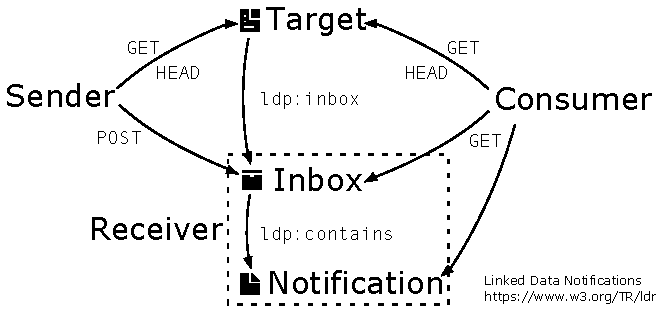
\includegraphics[width=0.8\textwidth]{images/ldn.pdf}
    \caption{Linked Data Notifications delivery model \cite{capadisli2017linked}. Note the different HTTP requests indicated using the arrows, as discussed in the text. Also note the discovery of the inbox and notifications using RDF predicates.}
    \label{fig:LDN}
\end{figure}

\noindent Van de Vyvere et al. \cite{van2020comparing} compare an HTTP polling approach with a push-based approach using \emph{Server-Sent Events (SSE)} on live Open Datasets. The datasets that are used are real-time in nature and most of them are almost continuously updated. The authors clearly show that, in order to minimize latency on the client, a push-based approach is required. When using these approaches, the server keeps the connection to the client alive, so that multiple updates of the dataset can be sent over the same connection. This practice eliminates the need for costly handshakes when initiating new connections and consequently benefits the performance. In addition to SSE, the authors also consider \emph{WebSockets}, which uses an HTTP handshake to initiate the channel, but further transmission occurs over a raw TCP connection that supports full-duplex bidirectional communication. SSE and WebSockets offer similar performance and since SSE is unidirectional and only reliant on HTTP, the former was chosen in this article. Moreover, the CPU usage of SSE in comparison to polling was also shown to decrease. In order to find a generic approach for all kinds of Linked Open Datasets, it is clear that some sort of pushing from the server should be supported to ensure support for fast-changing, continuously updating datasets.

\paragraph{WebSub}\cite{WebSub} \label{par:delivery-websub} is the last protocol considered in this section. This protocol was adopted by the W3C in 2018 and provides publish-subscribe communication using HTTP. Previously, this protocol was named \emph{PubSubHubbub}, because it uses the concept of \emph{hubs} as intermediary servers between publishers. These publishers own \emph{topics} and push updates to them, whereas they can be subscribed to by \emph{subscribers}. Subscribers need to be network-accessible at all times using their \emph{Subscriber Callback URL}. In order to subscribe to a topic, the subscriber sends an HTTP \texttt{POST}-request to a hub that contains their callback URL. For publishers, however, the specification does not provide a standardized way to update the hubs, hence it can be chosen by the developers. When a hub receives an update from a publisher, it notifies the subscribers by relaying the updates to their specified callback URL. The specification recommends that HTTPS is used at all times for HTTP requests and also specifies an additional \texttt{X-Hub-Signature} header that can be used for message authentication. This protocol might be of interest since it inherently supports decentralization, namely, hubs can be partitioned according to the needs of the user and so can the topic (i.e. topics can be duplicated across different hubs or could only be present on certain hubs). The downside to this protocol is that the subscribers must always be reachable via HTTP, which implies that the subscriber must operate a web server, to which updates can be pushed.